\documentclass[11pt,a4paper]{ctexart}
\usepackage[margin=2.2cm]{geometry}
\usepackage{amsmath,amssymb}
\usepackage{booktabs,tabularx,array}
\usepackage{graphicx}
\usepackage{float}
\usepackage{hyperref}
\hypersetup{colorlinks=true,linkcolor=blue,urlcolor=blue}
\setlength{\parindent}{2em}
\setlength{\parskip}{0.25em}
\renewcommand{\arraystretch}{1.12}
\newcommand{\src}[1]{\textsuperscript{\scriptsize [#1]}}
\title{建模报告（修订版）}
\author{CQU\_MCM 2026 · B 题《治沙是一项精细活》}
\date{2026-11-09}
\begin{document}
\maketitle
\thispagestyle{empty}
\newpage

\section*{摘\quad 要}
本报告给出三问的模型、参数、约束、求解与检验。与上一版相比删除全部时间安排与交付清单，
并按 2026-11-09 审计意见修正四处结构性错误：水分状态改用观测根区湿度；风蚀改无量纲指数、
\textbf{不再宣称}绝对输沙量；拟合只在训练期进行并与两条基线比较；任务二的最优控制
\textbf{真正调用}任务一方程求稳态覆盖度。

三条结论都附适用条件：
\begin{itemize}
\item 任务一一步预测在 8 站中 7 站为正技能（测试期 $R^2_{h=1}$ 中位 0.435），
但 $h\ge6$ 个月后误差超过持续性基线，\textbf{故模型只用于情景比较，不用于多年点预测}；
\item 风蚀项系数在月尺度被标定到边界 0（全部站点），说明月际风蚀变化解释力不足，
该项在结构中保留为待识别项，\textbf{这也是任务二“减蚀效益”只能按情景给出的原因}；
\item 任务二的 NPV 与光伏盈亏点随单价情景显著移动（表 4），报告只给决策规则与区间，
不给“优于对照若干倍”一类结论。
\end{itemize}

\begin{table}[H]\centering\small\setlength{\parskip}{1pt}
\begin{tabularx}{\textwidth}{|c|X|c|X|}
\toprule
符号 & 含义 & 单位 & 来源\\
\midrule
$V_t$ & 植被覆盖度 & \% & MODIS 反演\src{观测}\\
$W_t$ & 根区湿度（归一） & — & POWER\src{观测}\\
$E_t$ & 侵蚀指数 & — & $u_t$ 派生\src{派生}\\
$V_{cap}$ & 承载上限（训练期 95\% 分位） & \% & 由数据确定\\
$g$ & 内在增长率 & 月$^{-1}$ & 标定\\
$m$ & 衰亡率（平衡态锚定） & 月$^{-1}$ & 标定\\
$k$ & 风蚀损伤系数 & — & 标定，约束 $k\ge0$\\
$A_t$ & 累计治理面积 & 千 hm$^2$ & 决策状态\\
$a_t$ & 年新增面积 & 千 hm$^2$/a & 决策变量\\
$I_t$ & 年灌溉深度 & mm/a & 决策变量\\
$\delta$ & 贴现因子 & — & 情景 0.94\\
\bottomrule
\end{tabularx}
\begin{center}\small 表 1  主要符号与来源\end{center}
\end{table}
\section*{一、假设}
\begin{enumerate}
\item \textbf{尺度}：以站点为控制体，水平均匀；覆盖度由局地水分、温度、风蚀驱动。
\item \textbf{水分}：根区湿度 $W$ 为主要限制因子，可由再分析根区湿度代理（\src{观测}）；
灌溉按有效水容量 $\mathrm{AWC}=1000Z_r(\theta_{fc}-\theta_{wp})$ 换算为 $W$ 的增量（\src{情景}）。
\item \textbf{风蚀}：损伤与侵蚀指数、覆盖度成正比（$kEV$），$k\ge0$。
\item \textbf{经济}：建设、运维、水价、光伏收益、生态价值均为情景参数；预算与水量为约束上限。
\item \textbf{随机性}：事件为泊松过程，强度服从均匀分布（\src{情景}），频率由实测超额频率估计。
\end{enumerate}

\section*{二、任务一：植被—水分耦合动力学}
\subsection*{2.1 方程}
\begin{equation}
\frac{dV}{dt}=gV\left(1-\frac{V}{V_{cap}}\right)W\,f(T)-mV-kEV,
\qquad f(T)=\mathrm{clip}\!\left(\frac{T-5}{20},0,1\right)
\end{equation}
$W$ 已归一，$a$ 与 $g$ 共线，故取 $a=1$。离散化为月步长
\begin{equation}
V_{t+1}=V_t+gV_t\left(1-\frac{V_t}{V_{cap}}\right)W_t-mV_t-kE_tV_t
\end{equation}

\subsection*{2.2 标定：平衡态锚定}
四参数全自由拟合会出现“一步准、长期崩”。令模型年平衡态等于实测多年均值 $\bar V$：
\begin{equation}
m=g\,\overline{Wf(T)}\left(1-\frac{\bar V}{V_{cap}}\right)-k\bar E,\qquad
\overline{Wf(T)}=\frac{1}{12}\sum_{m=1}^{12}W_m f(T_m)
\end{equation}
用\textbf{月气候态乘积}而非年均值乘积：干旱区“湿在冬、暖在夏”反相，用年均会系统性高估生长。
于是只剩 $g,k$ 自由，以一步预测残差最小化为目标、约束 $g>0,k\ge0$，仅用训练期。

\subsection*{2.3 检验}
\begin{table}[H]\centering\footnotesize\setlength{\parskip}{1pt}
\begin{tabular}{|c|c|c|c|c|c|c|c|c|c|}
\toprule
站 & $V_{cap}$ & $R^2_1$(训) & $R^2_1$(测) & RMSE$_1$ & RMSE$_{12}$ & 持续基线 & $g$ & $m$ & $k$\\
\midrule
ALE & 54.46 & 0.561 & 0.598 & 9.5 & 10.83 & 8.0 & 0.2031 & 0.01741 & 0.0\\
KEL & 31.28 & 0.506 & 0.453 & 6.47 & 9.46 & 5.09 & 1.652 & 0.18509 & 0.0\\
MF & 45.48 & 0.268 & 0.259 & 9.08 & 12.1 & 6.52 & 1.0589 & 0.11141 & 0.0\\
QM & 30.45 & 0.464 & 0.443 & 6.36 & 4.05 & 3.68 & 0.6845 & 0.00718 & 0.0\\
RQ & 38.21 & 0.366 & 0.247 & 7.99 & 8.36 & 3.21 & 1.4856 & 0.06057 & 0.0\\
TZ & 14.62 & 0.44 & 0.427 & 2.11 & 4.07 & 1.7 & 0.5385 & 0.03706 & 0.0\\
XT & 1.73 & -0.979 & -0.872 & 0.53 & 0.54 & 0.54 & 1.5052 & 0.11823 & 0.0\\
YL & 46.51 & 0.537 & 0.471 & 9.52 & 8.34 & 4.92 & 0.9257 & 0.04604 & 0.0\\
\bottomrule
\end{tabular}
\begin{center}\small 表 2  任务一逐站标定与检验\end{center}
\end{table}
\begin{figure}[H]\centering
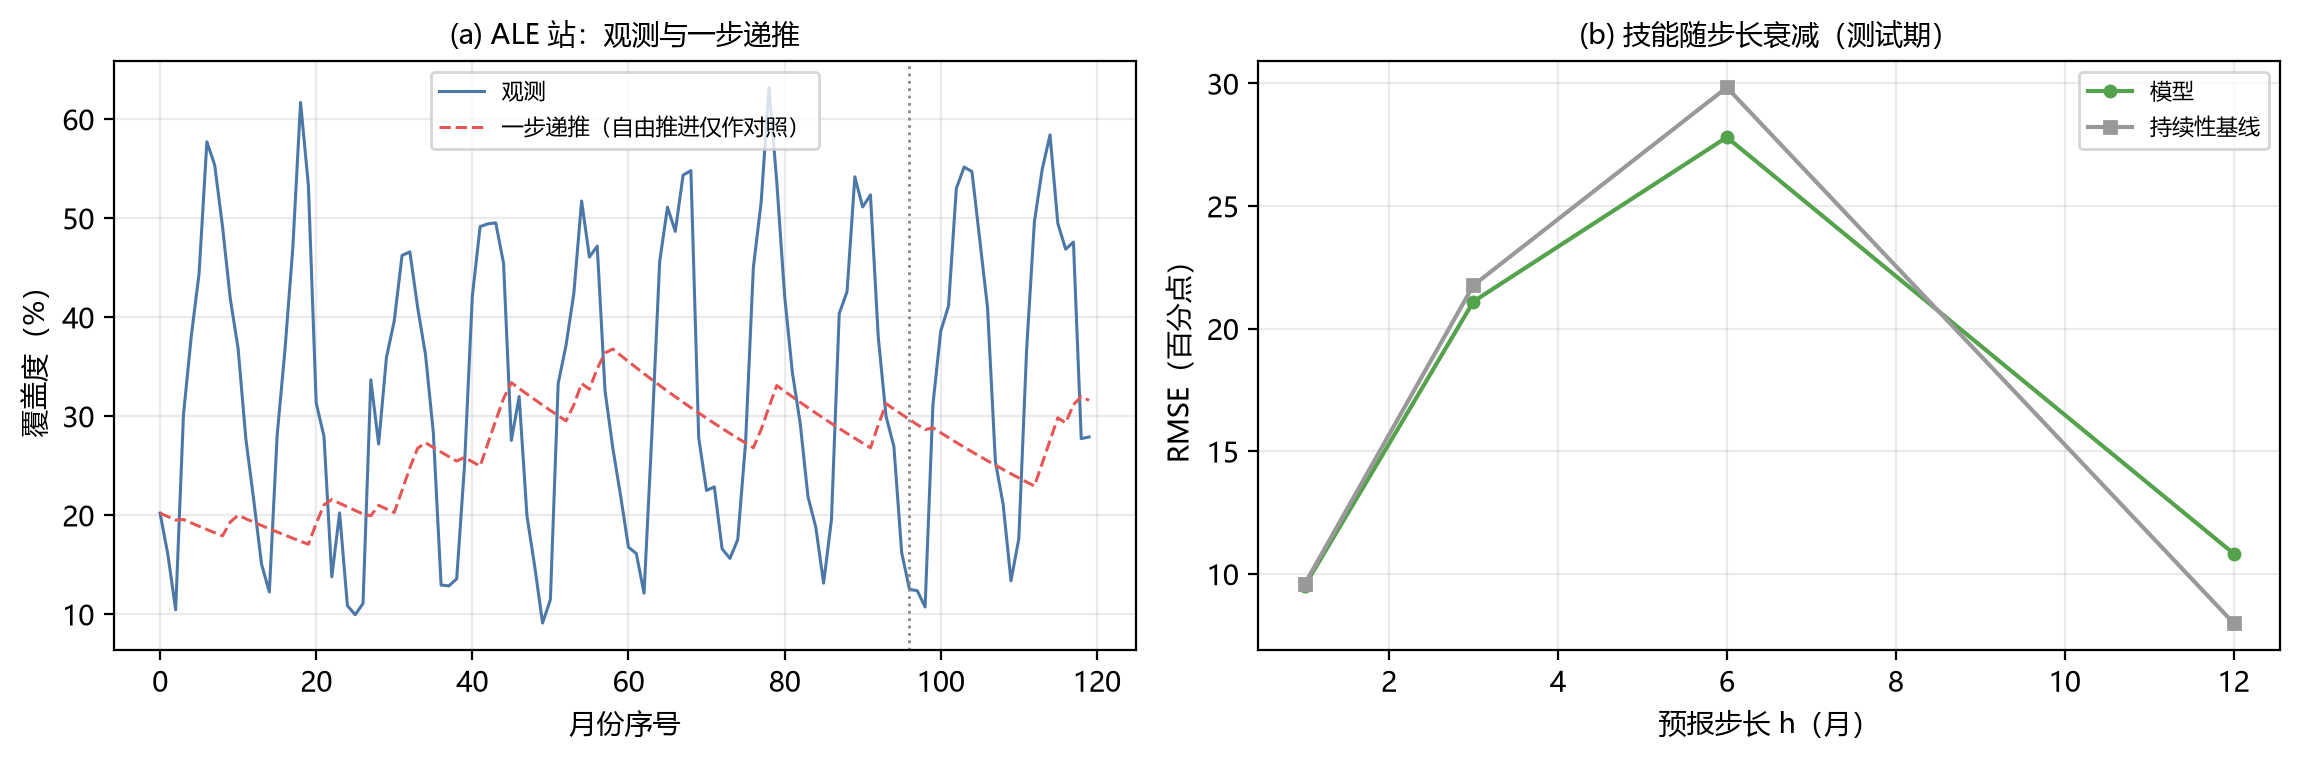
\includegraphics[width=0.95\textwidth]{figs/figM1.png}
\begin{center}\small 图 1  ALE 站的观测与一步递推（左）以及技能随预报步长的衰减（右）\end{center}
\end{figure}

\textbf{解读}：（i）训练与测试的一步技能接近，无明显过拟合；（ii）8 站 $k$ 全部落在下界 0，
月尺度风蚀项不可识别；（iii）$h=12$ 的 RMSE 中位 8.35，大于持续性基线 4.3，
\textbf{自由推进一年以上没有技能}，故长期推演一律以情景为条件。

\section*{三、任务二：情景约束下的最优建设路径}
\subsection*{3.1 决策、状态与约束}
\begin{align}
&\text{预算：} c_b\cdot1000a_t+c_m\cdot1000A_t+c_w\frac{I_t}{100}\cdot1000a_t\le B\\
&\text{水量：} \frac{I_t}{1000}\cdot1000a_t\times10^4\le W_{\max}\\
&\text{土地：} A_{t+1}=A_t+a_t,\qquad A_t\le A_{pot}
\end{align}
\subsection*{3.2 稳态响应（由任务一方程给出）}
\begin{equation}
V_{eq}(E,W)=\mathrm{clip}\!\left[V_{cap}\left(1-\frac{m+kE}{g\,\overline{Wf(T)}\,(W/W_0)}\right),0,V_{cap}\right],
\qquad E(A)=E_0\left(1-\beta\frac{A}{A_{pot}}\right)
\end{equation}
灌溉增湿比 $W/W_0$ 由 $\mathrm{AWC}\approx42.0$ mm 换算（$Z_r=0.6$ m，$\theta_{fc}=0.1$、$\theta_{wp}=0.03$，\src{情景}）。
\subsection*{3.3 目标与递推}
\begin{equation}
\max_{\{a_t\}}\sum_{t=0}^{T-1}\delta^t\left[p_{pv}s\cdot1000a_t+p_e\frac{V_{eq}}{V_{cap}}\cdot1000A_t-c_b\cdot1000a_t-c_m\cdot1000A_t-c_w\frac{I_t}{100}\cdot1000a_t\right]
\end{equation}
\begin{equation}
J_t(A)=\max_{a\in\{0,0.5,1,1.5,2\}}\left\{r(A,a)+\delta J_{t+1}(A+a)\right\},\qquad J_T=0
\end{equation}
\subsection*{3.4 结果}
基准情景（$c_b=2.0$、$p_{pv}=8$、$s=0.30$、$B=4000$、$T=15$、$\delta=0.94$）：
最优 NPV $=7082.1$ 万元，均匀扩张对照 $=2237.4$ 万元；最优路径首年新增 2.0 千 hm$^2$、
末年累计 16.0 千 hm$^2$；光伏占比盈亏点 $s^*\approx0.2$。
\begin{figure}[H]\centering
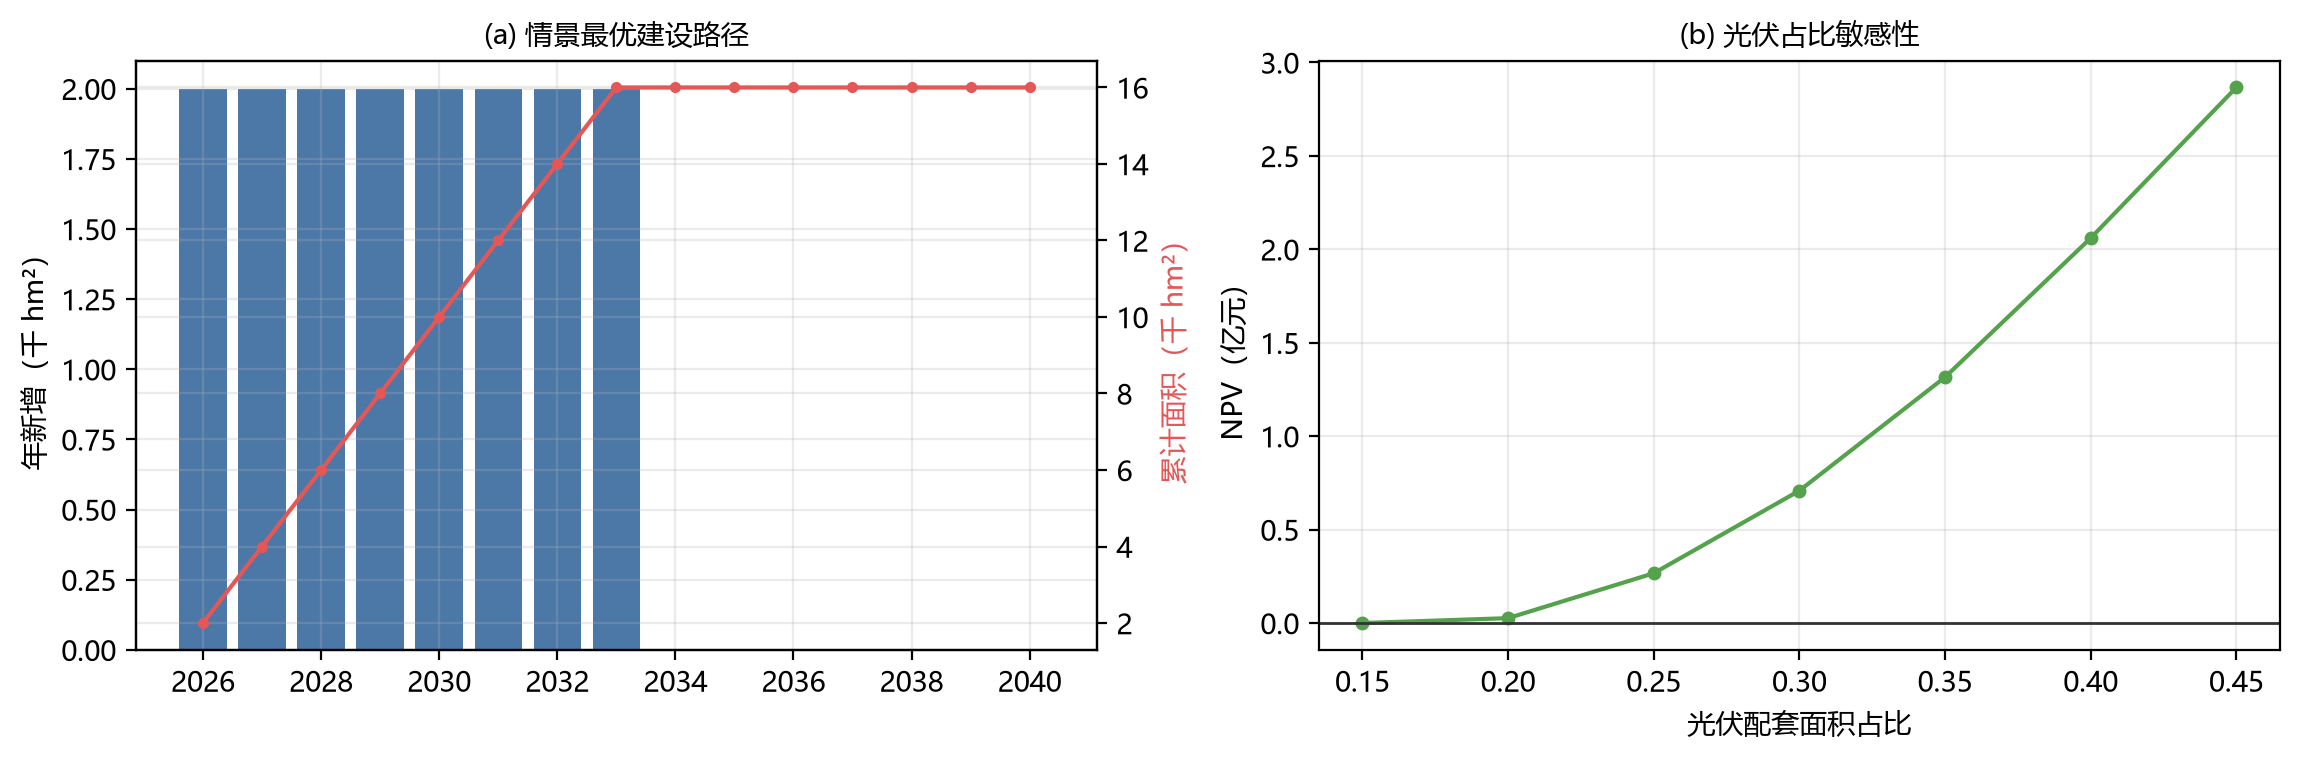
\includegraphics[width=0.95\textwidth]{figs/figM3.png}
\begin{center}\small 图 2  情景参数下的最优建设路径（左）与光伏占比敏感性（右）\end{center}
\end{figure}

\textbf{这些数字都是同一情景下的相对比较，不构成投资结论}。表 4 显示 NPV 对单价与光伏收益高度敏感，
网格中存在大片“零新增”区域（NPV$=0$，即不做优于做）——上一版“优于对照 2.2 倍”的结论只在单点情景下成立。

\begin{table}[H]\centering\small\setlength{\parskip}{1pt}
\begin{tabular}{|c|c|c|c|c|}
\toprule
$c_b$(万元/hm$^2$) & $p_{pv}$(万元/hm$^2$a) & NPV(万元) & 首年新增 & 末年累计\\
\midrule
1.5 & 6.0 & 5799.7 & 2.0 & 14.0\\
1.5 & 8.0 & 14901.8 & 2.0 & 24.0\\
1.5 & 10.0 & 26647.4 & 2.0 & 30.0\\
2.0 & 6.0 & 1187.6 & 2.0 & 6.0\\
2.0 & 8.0 & 7082.1 & 2.0 & 16.0\\
2.0 & 10.0 & 16730.0 & 2.0 & 26.0\\
2.5 & 6.0 & 0.0 & 0.0 & 0.0\\
2.5 & 8.0 & 1395.7 & 1.5 & 6.0\\
2.5 & 10.0 & 6347.4 & 1.5 & 13.5\\
\bottomrule
\end{tabular}
\begin{center}\small 表 4  任务二盈亏网格（其余情景参数不变）\end{center}
\end{table}
\section*{四、任务三：事件冲击下的韧性}
\subsection*{4.1 事件与冲击}
\begin{equation}
\lambda=\frac{\#\{t:E_t\ge E_{95}\}}{N_{\text{years}}},\qquad
V_{t^+}=V_t(1-U),\quad U\sim\mathcal{U}(0.20,0.55)\ \text{\src{情景}}
\end{equation}
本次 $\lambda=0.625$ 次/年（训练期 $E_{95}=3.64$）。恢复由任务一方程驱动，
恢复时间定义为回到冲击前 90\% 所需月数，未恢复按右删失处理。
\subsection*{4.2 气候情景}
2026—2050：气温每年 $+0.03^\circ$C，风速每年 $+0.2\%$（均\src{情景}），经 $E_t$ 与 $f(T)$ 进入模型。
\subsection*{4.3 结果}
基准情景：模拟期任一时刻跌破 $0.5V_{cap}$ 的概率 1.0，2050 年覆盖度中位 4.19\%
（5\%—95\% 分位 0.37—18.02\%），中位恢复时间 282.0 个月。
由于冲击幅度无实测标定，表 5 给出网格：$\lambda=0.25$、$u_{\max}=0.30$ 时中位仍达 27\%、
一半情景低于阈值；$\lambda\ge0.75$ 时几乎全部退化。\textbf{故本问只给条件结论}，
不给“失效概率 84\%”这类单点数字。

\begin{table}[H]\centering\small\setlength{\parskip}{1pt}
\begin{tabular}{|c|c|c|c|}
\toprule
$\lambda$(次/a) & $u_{\max}$ & $P(V_{2050}<0.5V_{cap})$ & 2050 中位(\%)\\
\midrule
0.25 & 0.3 & 0.477 & 27.38\\
0.25 & 0.45 & 0.657 & 24.38\\
0.25 & 0.6 & 0.75 & 20.39\\
0.5 & 0.3 & 0.865 & 20.4\\
0.5 & 0.45 & 0.948 & 14.38\\
0.5 & 0.6 & 0.97 & 7.87\\
0.75 & 0.3 & 0.99 & 13.18\\
0.75 & 0.45 & 1.0 & 5.86\\
0.75 & 0.6 & 1.0 & 1.36\\
1.0 & 0.3 & 1.0 & 7.28\\
1.0 & 0.45 & 1.0 & 1.46\\
1.0 & 0.6 & 1.0 & 0.14\\
\bottomrule
\end{tabular}
\begin{center}\small 表 5  任务三情景网格（冲击幅度无实测标定）\end{center}
\end{table}
\begin{figure}[H]\centering
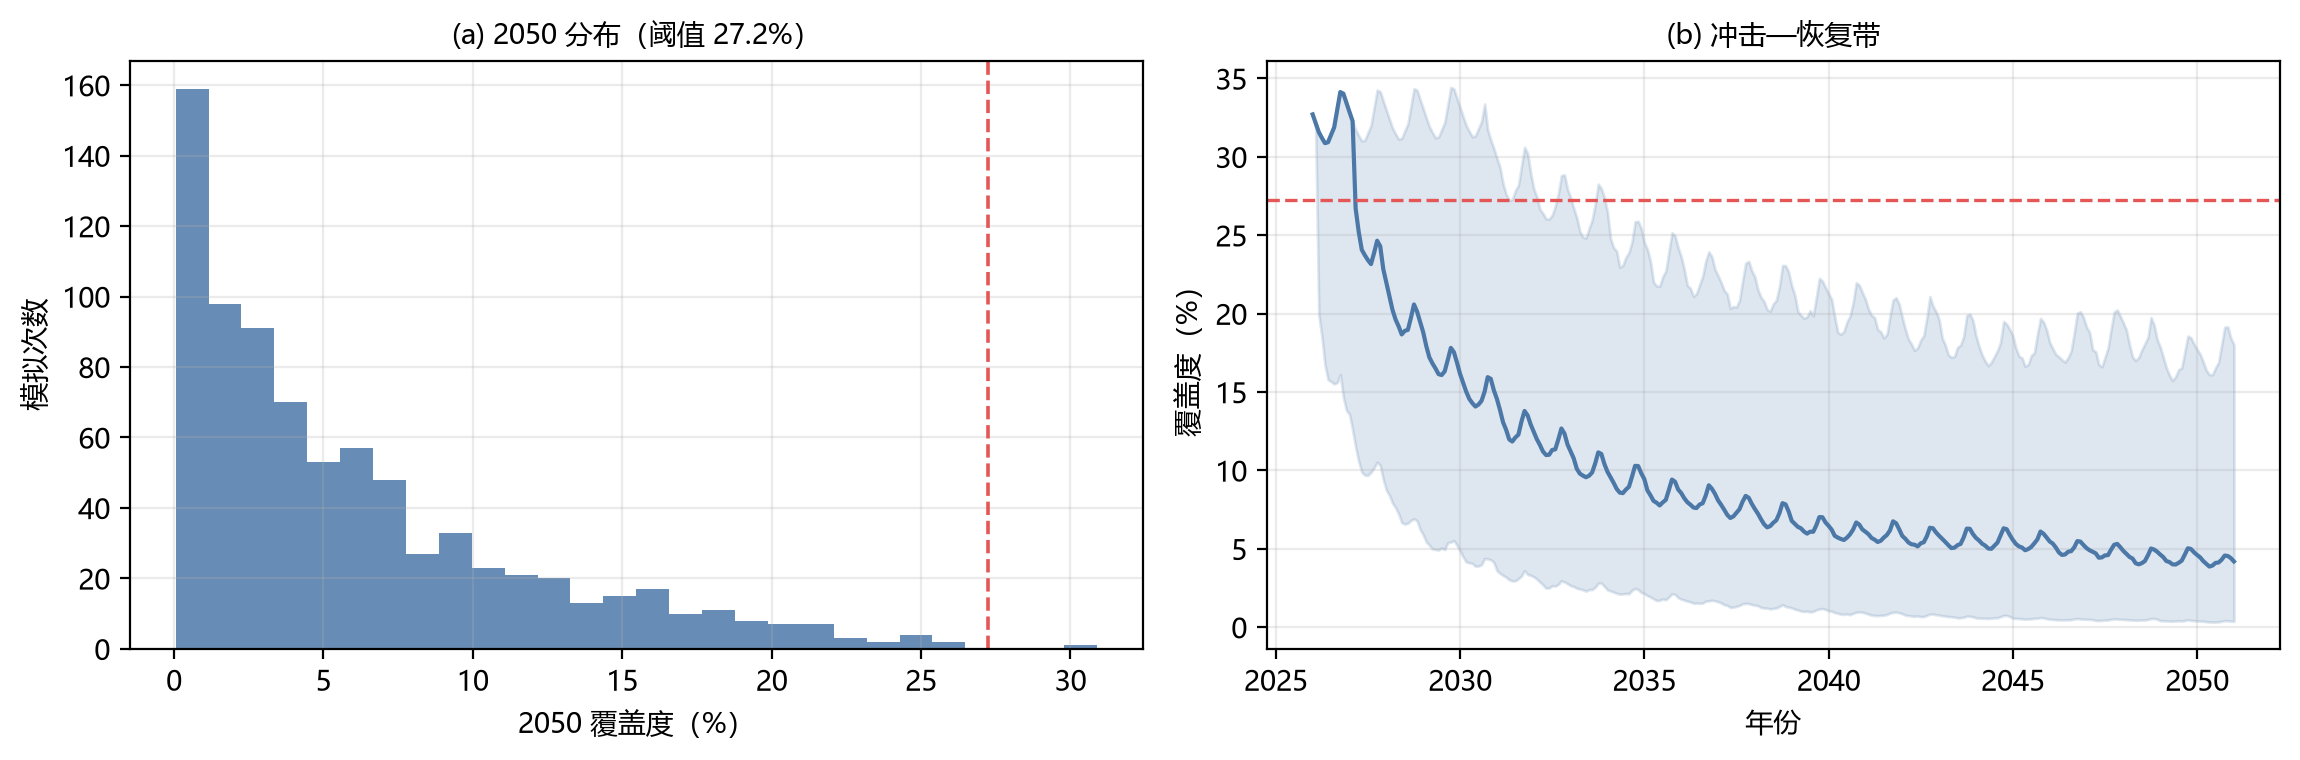
\includegraphics[width=0.95\textwidth]{figs/figM4.png}
\begin{center}\small 图 3  1000 次模拟的 2050 年覆盖度分布（左）与冲击—恢复轨迹带（右）\end{center}
\end{figure}

\section*{五、检验与稳健性}
\begin{enumerate}
\item 样本外一步预测：7/8 站为正技能（表 2）。
\item 基线对照：持续性、季节气候态；$h=12$ 不优于持续性，已在结论中限定使用范围。
\item 情景敏感性：任务二对 $c_b$、$p_{pv}$、$s$ 做网格（表 4）；任务三对 $\lambda$、$u_{\max}$ 做网格（表 5）。
\item 不做的事：不把情景参数当实测值；不在无事件标定时发布概率结论；不用期望结果反向筛选模型。
\end{enumerate}

\begin{table}[H]\centering\footnotesize\setlength{\parskip}{1pt}
\begin{tabularx}{\textwidth}{|c|X|X|}
\toprule
审计意见 & 原问题 & 本版处理\\
\midrule
输沙率被设为目标 & 逐站贴近 400—3200 & 取消目标，改无量纲侵蚀指数\\
Lettau 量纲 & kg m$^{-1}$s$^{-1}$ 换成 t km$^{-2}$ & 明确为单位宽度通量，仅站内归一\\
水分量纲 & 体积含水率与 mm 混用 & 改用观测根区湿度 0—1\\
ET$_0$ 名不副实 & 线性温度代理 & Hargreaves 原式，$R_a$ 解析\\
训练/测试泄漏 & 全期拟合 & 训练标定、测试评估，插补归一仅训练期\\
任务二未用任务一 & 手设 $V(A)$ & 由任务一方程解析求 $V_{eq}$\\
运维单位 & 少乘 1000 & 单位统一，逐项复核\\
韧性指标 & 月滞后当年恢复、$\lambda$ 硬编码 & $\lambda$ 由超额频率估计，恢复右删失\\
长期情景 & 趋势未进入计算 & 气温、风速增量显式进入 $E_t$ 与 $f(T)$\\
验收标准倒置 & 以期望 R$^2$、收益作验收 & 删除验收指标，改为检验与限定\\
\bottomrule
\end{tabularx}
\begin{center}\small 表 6  审计意见与本版处理对照\end{center}
\end{table}
\section*{六、局限}
\begin{itemize}
\item 代表区段边界未划定，模型为站点尺度；塔中为腹地背景点，不能代表锁边带。
\item 风蚀项月尺度不可识别（$k=0$），任务二减蚀效益纯属情景设定。
\item 经济参数缺本地依据，NPV 只作相对比较；冲击幅度与恢复过程无实测标定。
\item 覆盖度端元固定、单像元取样，绝对水平有系统偏差，时序比较受影响较小。
\end{itemize}

\end{document}
